\subsection{User comments}

This section includes first-person accounts from two members of our team who implemented data consistency for the same e-commerce prototype, respectively.

\paragraph{Eventuate (Nana)}

\begin{itemize}
    \item \textit{Pros \#1}: Eventuate framework maintains high modularity by dependency injection, using tags such as \texttt{@even\-tentity}, \texttt{@event}, \texttt{@aggregate}, \texttt{@eventsubscriber} to define unit field. Each of these fields has a generic abstract class to inherit, which makes user easier to organize system structure. Decoupling is one of the benefits in modularity. Due to the high modularity in Eventuate, it also has low coupling as well.
    \item \textit{Pros \#2}: Eventuate persists transaction atomicity by using sequence of state-changing events in entity. Whenever the state of a business entity changes, a new event is appended to the list of events. Eventuate workflow includes command processing and event publishing while updating entity status. This design reconstructs an entity’s current state by replaying the events. Since saving an event is a single operation, it is inherently atomic.
    \item \textit{Pros \#3}: Eventuate provides clean and concise samples for users to start up their application. Those samples have great code legacy in modularity, which divides a large system into different layers and helps user to find useful information efficiently.
    \item \textit{Cons \#1}: Eventuate is difficult to configure or saying, difficult to configure without Docker. Unlike Axon, which could download the released package and run locally, Eventuate provides services through Docker and Docker Compose. Therefore, it requires user to learn how to use Docker first. Eventuate also provides free AWS platform to run their services without local configuration. But it takes them 2 weeks to respond my request for AWS access key, which is quite slow.
    \item \textit{Cons \#2}: One key drawback of Eventuate is that it uses too many extra products such as Zookeeper and Kafka to implement functionality. In our system, we have implemented 4 services but using Eventuate requires 5 extra services to run first. The resource consumption such as CPU utilization is higher than Axon. Also, during our experiment, we found that some services in Eventuate is not stable and often stop running in Docker automatically. It is possible that Eventuate has bug not found, which makes it unstable or not compatible with Docker.
    \item \textit{Cons \#3}: Even though the sample code is well organized in Eventuate, its tutorial is worse than Axon or any other framework tutorial I have read before. The documentation merely defines the syntax of the API, but \textbf{not} the underlying semantics – the intents of the functions and their effects on the whole system. Also, the tutorial covers only a small section of implementation in Eventuate. For example, EventUtil is frequently used in sample code but never explained in tutorial.
\end{itemize}

\paragraph{Axon (Xin)}

\begin{itemize}
    \item \textit{Pros \#1}: Building with Axon is highly modular, each entity or a type of entities is represented by an aggregate. Inside a aggregate class, we declare its attributes and aggregate id. \texttt{Commands} and \texttt{Events} are also classes that capture what actions to take. Axon extensively provide annotation support, such as \texttt{@aggregate}, \texttt{@commandHandler}, \texttt{@eventSourcing}, which made it easy to the developers.
    \item \textit{Pros \#2}: Axon official website \cite{axon} has documentations that explain terminologies and provide code samples. It is a well-documented framework, and updates regularly.
    \item \textit{Pros \#3}: Configuration with Spring is also easy. Spring is not a prerequisite for using Axon, so developers have the flexibility to make their own decision based on personal preference.
    \item \textit{Pros \#4}: Axon is open-source and freely available, there are big organizers such as banks using Axon in their core system. This also indicates that Axon is a fairly mature framework.
    \item \textit{Cons \#1}: Hard to handle mistakes in event handlers locally: if an error appears in one of the event handlers, there is no other way than reconstructing past states. The replaying process may take a long time depending on data size.
    \item \textit{Cons \#2}: Since commands and events are immutable, they have to be defined by Kotlin (Kotlin is a statically typed programming language that runs on the JVM and also can be compiled to JavaScript source code or use the LLVM compiler infrastructure.) and put into core api. Although Kotlin allows users to concisely define each event and command on a single line, it may add extra work for people who has no experience with Kotlin.
\end{itemize}


\subsection{Code examples}

\begin{figure}[H]
    \centering
    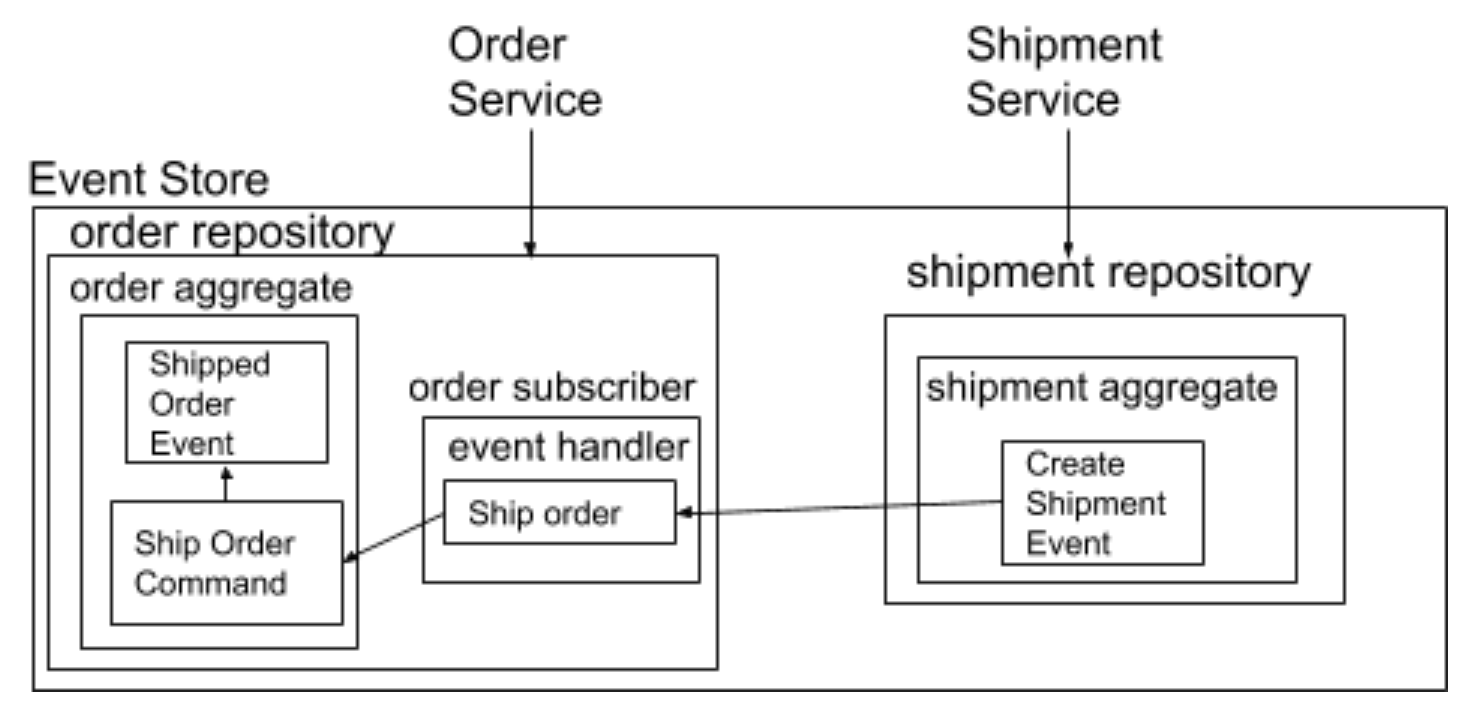
\includegraphics[width=9cm]{assets/README-d8970.png}
    \nocaptionrule \caption{\label{fig:code-example} Content in event store for shipping and ordering service}
\end{figure}

\subsubsection{Eventuate}
\begin{enumerate}[i]
    \item Create basic components of the service: \texttt{ShipOrderCommand}, \texttt{OrderShippedEvent}, and \texttt{ShipmentCreated\-Event}. (Listing \ref{code:eventuate-basic} in Appendix)
    \item Set up event handler method in order service to monitor \texttt{ShipmentCreatedEvent} and invoke \texttt{ShipOrder\-Command} if \texttt{ShipmentCreatedEvent} is generated. (Listing \ref{code:eventuate-handler})
    \lstinputlisting[language=java, caption={Event handler example in Eventuate}, label=code:eventuate-handler]{code/even-handler.java}
    \item Overload \texttt{process} function in \texttt{ShipOrderCommand} class and \texttt{apply} function in \texttt{OrderShippedEvent} class in \texttt{Order} aggregate to generate \texttt{ShipmentCreatedEvent} and change order status. (Listing \ref{code:eventuate-event})
    \lstinputlisting[language=java, caption={Overloading \texttt{apply} and \texttt{process} in Eventuate}, label=code:eventuate-event]{code/even-event.java}
\end{enumerate}

\subsubsection{Axon}

\begin{enumerate}[i]
    \item Basic unit is aggregate. An aggregate is an entity or a collection of entities. It needs to have an aggregate id.

    \lstinputlisting[language=java, caption={\texttt{Aggregate} example in Axon}, label=code:eventuate-handler]{code/axon-aggregate.java}

    \item Command classes are identified by the aggregate id it relates to.

    \lstinputlisting[language=java, caption={\texttt{Command} example in Axon}, label=code:eventuate-handler]{code/axon-command.java}

    \item Each aggregate defines their own commandHandlers, each eventSourcingHandler corresponds to one type of commandHandler. For the example below, we assign orderId to this order object only if the command is of type \texttt{FileOrderCommand}.

    \lstinputlisting[language=java, caption={Handlers defined in Axon}, label=code:eventuate-handler]{code/axon-handler.java}

    \item After the order goes through, Shipment aggregate will receive \texttt{prepareShipmentCommand}, and apply \texttt{ShipmentPreparedEvent} for this order.
    \lstinputlisting[language=java, caption={Shipment aggregate in Axon}, label=code:eventuate-handler]{code/axon-ship.java}

    \item The eventSourcingHandler for \texttt{ShipmentPreparedEvent} is called after applying the event successfully in the commandHandler.
    \lstinputlisting[language=java, caption={Shipement event handler in Axon}, label=code:eventuate-handler]{code/axon-eventsource.java}
\end{enumerate}

\subsection{Load test and Resource Consumption}

\begin{table}[H]
    \begin{center}
        \begin{tabular}{ | m{2cm} | l | l | }

            \hline
            & Axon & Eventuate \\

            \hline
            CPU Utilization &
            $66.4\%$ &
            $19.6\%$ \\

            \hline
            Median Request Latency &
            $58.4$ ms &
            $345.6$ ms \\

            \hline
            Service Breakdown & No & Yes \\

            \hline

        \end{tabular}
    \end{center}
    \caption{Comparison between Axon and Eventuate}
    \label{table:load}
\end{table}

To test for the \textbf{stability} of Axon and Eventuate, we used Artillery to load-test the prototypes. Since data consistency is guaranteed by the framework and thus is not the central concern for this particular test, we only test for a part of the whole purchase transaction: \textit{assuming an existing user, place an order with the ID of that user}. In this test, we repeatedly create new orders under the same customer and test whether the system can handle the traffic load. In the load-test for Eventuate, \textbf{12000} requests are sent within 120 seconds, and all request succeeded. However, the same load completely broke the Axon version of the same prototype. Note that although the requests were never successful, no partial transactions were performed by Axon, and the system is indeed consistent. Therefore, Axon was tested using fewer number of requests. The results are summarized in Table \ref{table:load}.

\subsection{Development tatistics}

The following table summarizes statistics about the two prototypes and development of them. Fully LOC information can be found in Appendix (Listings \ref{code:eventuate-loc}, \ref{code:axon-loc}).

\begin{table}[H]
    \begin{center}
        \begin{tabular}{ | m{2cm} | l | l | }

            \hline
            & Axon & Eventuate \\

            \hline
            Total Time Spent &
            $41.3$ hours &
            $63.5$ hours \\

            \hline
            LOC (Java) &
            1189 lines &
            2304 lines \\

            \hline
            LOC (Total) &
            2300 lines &
            3227 lines \\

            \hline

        \end{tabular}
    \end{center}
    \caption{Development statistics of two prototypes}
    \label{table:stats}
\end{table}

During the development, we also attempted to search on \texttt{http://stackoverflow.com/} for either Axon or Evantuate related questions, As of May 4, 2018, searching or ``Axon'' gives \textbf{336} results\footnote{https://stackoverflow.com/search?q=axon}, whereas searching for ``Eventuate'' gives \textbf{51} results\footnote{https://stackoverflow.com/search?q=eventuate}.
